\documentclass[assignment06_Solutions]{subfiles}

\IfSubStr{\jobname}{\detokenize{Solutions}}{\toggletrue{solutions}}{\togglefalse{solutions}}
%\IfSubStr{\jobname}{\detokenize{Solutions}}{\toggletrue{solutions}}{\toggletrue{solutions}}

\fancypagestyle{firstpage}

{\rhead{Assignment 6 \linebreak \textit{Version: \today}}}

\title{Assignment 6: Introduction to Neural Networks and Backpropagation}
\author{Machine Learning}
\date{Fall 2021}

\begin{document}

\maketitle
\thispagestyle{firstpage}


\begin{learningobjectives}
\bi
\item Understand the difficulties that neural networks address in comparison to algorithms like logistic regression.
\item Interpret the results of applying a simple neural network to a dataset.
\item Understand the architecture of a particular type of neural network called a multi-layer perceptron.
\item Learn how to represent the multivariable chain rule graphically.
\item Understand how the backpropagation algorithm can be used to compute the gradient of a loss function with respect to the parameters of a neural network.
%\item Learn about a few strategies used to optimize the weights of a neural network that leverage the gradient of the loss function with respect to the network's parameters.
\ei
\end{learningobjectives}


\section{Assignment Structure}
In this assignment we'll be doing the following things in order to meet the learning goals articulated above.
\be
\item Motivate the idea of neural networks through a Jupyter notebook that examines the \href{https://www.kaggle.com/c/titanic}{Titanic Dataset from Kaggle}.
\item Introduce the architecture of a particular type of neural network called a multi-layer perceptron.
\item See another way to think about the chain rule for multivariable functions that uses a graphical representation.
\item Learn about, and ultimately derive, the backpropagation algorithm.
\ee

\begin{priorknowledge}
Here are some things we'll be utilizing in this assignment.  When appropriate, we'll call these out in a particular section with some helpful text to jog your memory.
\bi
\item Logistic regression algorithm
\item Multivariable chain rule
\item Binary classification problem setting
\ei
\end{priorknowledge}

\section{Motivation for Neural Networks}

In order to motivate the idea of neural networks, we'll be examining the \href{https://www.kaggle.com/c/titanic}{Titanic Dataset from Kaggle}. This dataset is commonly used in machine learning examples. We'll just be taking a quick look at it, using only two traits to try to predict whether or not someone survived the shipwreck.

\vspace{1em}
\begin{externalresources}[(45 minutes)]
Go through the \href{https://colab.research.google.com/drive/137d9N0jnsVqlKIwDFUy3zauIXx9UDIOr?usp=sharing}{Assignment 6 Companion notebook}.
\end{externalresources}

\section{Our First Neural Network: the Multilayer Perceptron (MLP)}

Now that you've seen a neural network in action, we'll be digging into how a neural network works.  The presentation will be specific to a particular type of neural network that we used in the companion notebook known as a multilayer perceptron (MLP), but the main ideas generalize to many other types of networks.

Thinking back to the companion notebook, we observed that the features in the original dataset ({\tt age} and {\tt sex}) were not conducive to predicting whether someone would survive.  We showed that by augmenting the input features with a column called {\tt is young male} that captured whether or not a person was young \emph{and} male, that the algorithm could effectively learn the task.  The fundamental idea of a neural network is that the network automatically constructs useful representations of the input data \emph{as a part of the learning process}.

Graphically we can contrast these approaches in the following way.  First we'll show the logistic regression model that we applied in the notebook.

\includegraphics[width=\linewidth]{figures/titaniclogisticregression}\marginnote{To interpret these diagrams, think of the circles (also called nodes) as representing values that are either input to or computed by the network.  Directed lines (also called edges) represent data flowing in the network.  Each edge multiplies the value flowing into it by a weight (represented by a text label on the edge).}

Notice how we had to manually introduce the feature {\tt is young male} in order for the logistic regression model to utilize it to make its prediction.  Before giving you the equivalent figure for the multi-layer perceptron, let's look at a little bit more cartoonish version of the multi-layer perceptron.  This version will leave off the math and the particular notation we are using.  Once you have a good sense of what this is, you can look at the more precise version which is to follow.


\begin{externalresources}{(optional)}
Here are some additional resources that explain the concept of a multi-layer perceptron.  If the explanations we give below are not working for you, consider checking out some of these.  \textbf{You do not need to consult these resources if you feel like our explanations are working well for you.}
\bi
\item 3blue1brown \href{https://www.youtube.com/watch?v=aircAruvnKk&t=6s}{What is a neural network?} 
\item 3blue1brown video \href{https://www.youtube.com/watch?v=IHZwWFHWa-w&list=PL_h2yd2CGtBHEKwEH5iqTZH85wLS-eUzv&index=2}{How neural networks learn?}
\item 3blue1brown \href{https://www.youtube.com/watch?v=Ilg3gGewQ5U}{Backpropagation}
\ei
\end{externalresources}

\includegraphics[width=\linewidth]{figures/titanicmlpsimple}

Input data (in this case we just use age, male, and a bias term) are propagated via a set of connection weights to a set of hidden representations.  These hidden representations are propagated via another set of a connection weights to the output of the network.   In the companion notebook we showed that for the Titanic dataset, the network learned two hidden representations: one that seemed to encode {\tt is young male} and the another that encoded sex.  Of particular importance is that we did not have to manually introduce the {\tt is young male} feature.

Next, let's make this cartoon picture concrete.  We'll use the following notation.
\bi
\item $x^{(k)}_i$ will refer to the $i$th unit in the $k$th layer of the network ($k=1$ will correspond to the inputs, $k=2$ will correspond to the hidden representations, and $k=3$ will correspond to the output).  For instance, in the figure above the circle labeled \emph{male} would be $x^{(1)}_2$, \emph{hidden repr. 1} would be $x^{(2)}_1$ and \emph{prob survived} would be $x^{(3)}_1$.
\item $s^{(k)}_i$ will refer to the $i$th summation unit in the $k$th layer of the network (as before, $k=1$ will correspond to the inputs, $k=2$ will correspond to the hidden representations, and $k=3$ will correspond to the output).  The summation unit will play a similar role to $s$ in the logistic regression figure.
\item $w^{(k)}_{i,j}$ will refer to the weight of the connection between the the $j$th unit in layer $k$ and the $i$th unit in layer $k+1$.
\ei

\begin{notice}
There are a lot of symbols here!  Take some time to unpack each of them.  Make sure you know what superscripts and subscripts represent.  While there is an upfront cost to introducing these symbols, it will ultimately make the derivation of the general form of the MLP easier.
\end{notice}
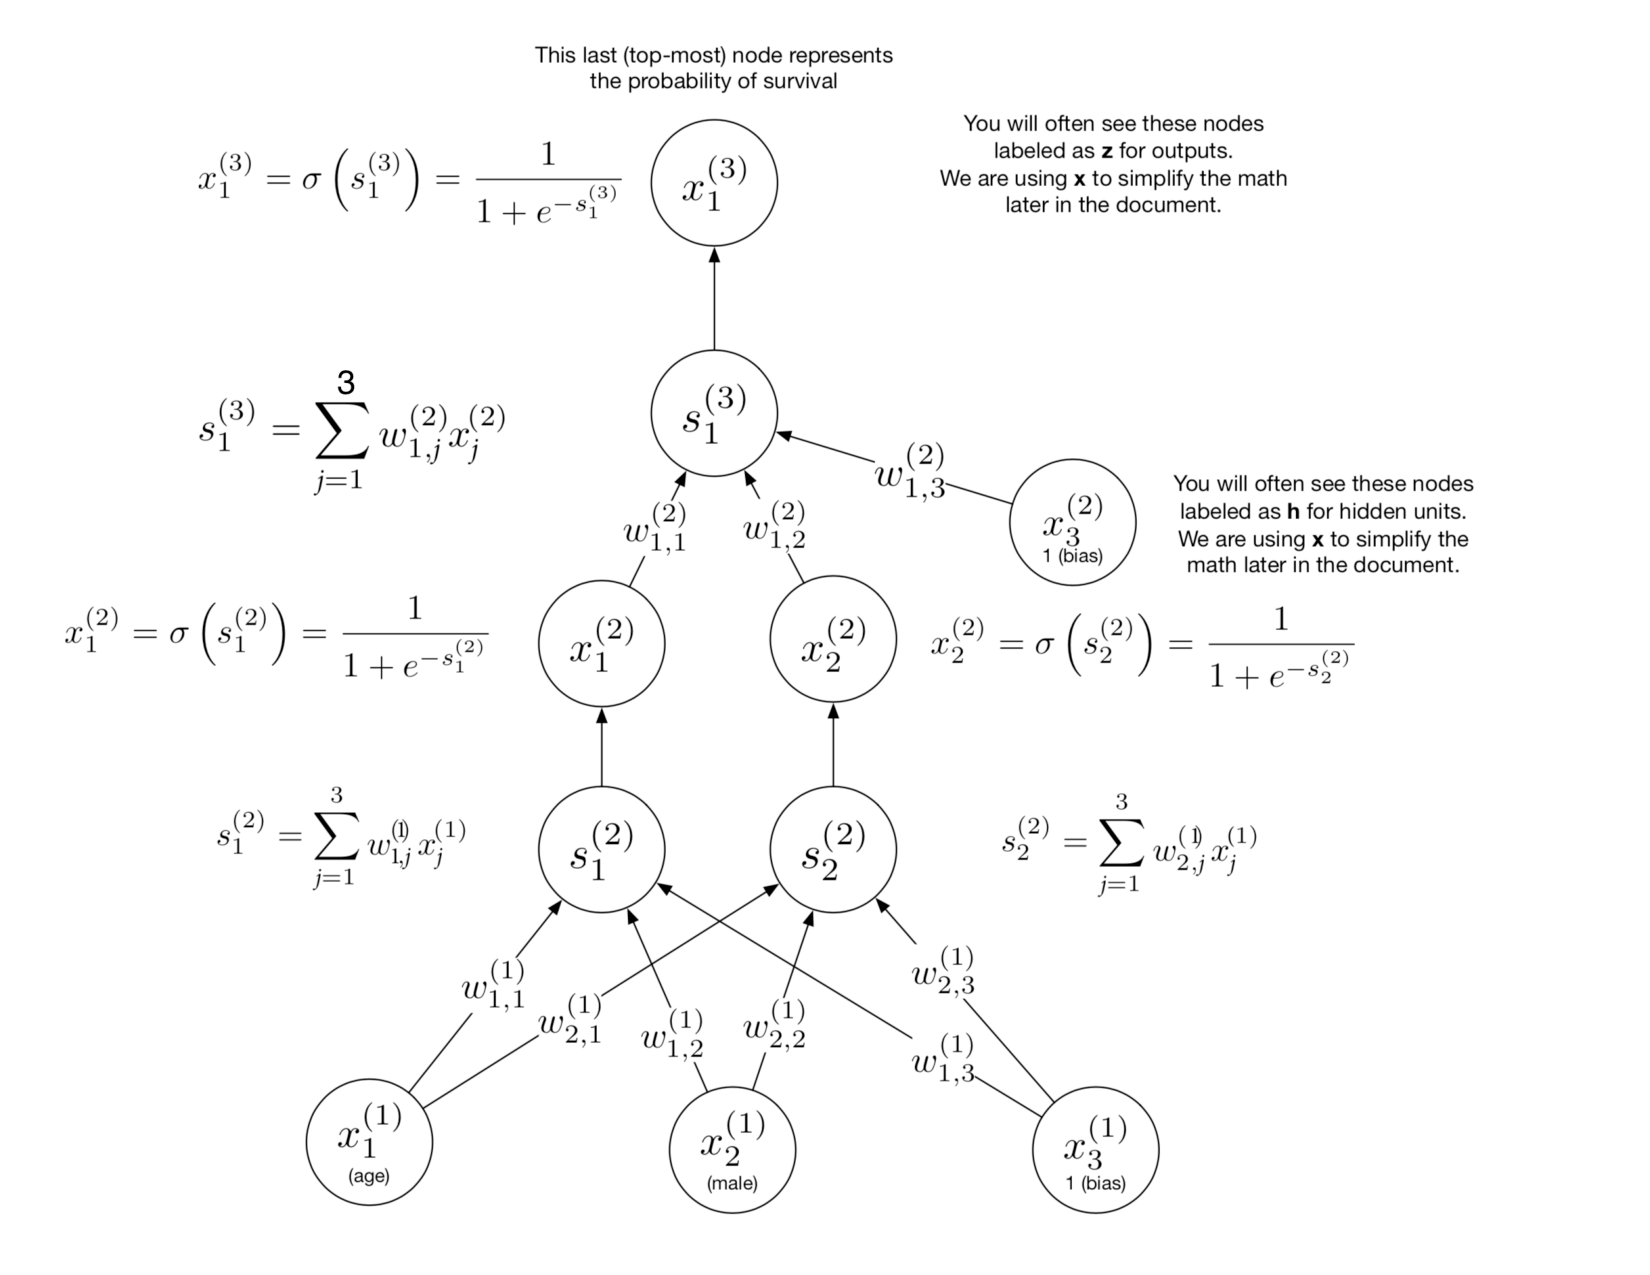
\includegraphics[width=\linewidth]{figures/titanicmlp2}

\vspace{1em}

\begin{exercise}[(10 minutes)]
Before going on, let's make sure you have a firm handle on what's being represented in the figure above.
\bes
\item Just as in logistic regression, we will try to tune the weights to fit the data.  How many weights are there to tune in this network?
\begin{boxedsolution}
There are a total of 9 weights in the network.  There are 6 connecting the 3 input units to the 2 hidden summation units.  There are another 3 connecting the 1 output summation unit.
\end{boxedsolution}
\item While the figure looks pretty crazy, it has a lot of similarities with the logistic regression model.  Where does the logistic regression model show up in the figure?
\begin{boxedsolution}
There are three different logistic regression models represented.  There is one going from the inputs to the $x_1^{(2)}$.  There is another going from the inputs to $x_2^{(2)}$.  There is a third going from the hidden units to $x_1^{(3)}$.  The models are connected together such that the two lower logistic models feed into the higher-level one.
\end{boxedsolution}
\ees
\end{exercise}

\begin{exercise}[(30 minutes)]
For each of the 3 behavors described below (questions a, b, and c), determine reasonable values for the weights in this network ($w^{(1)}_{1,1}, w^{(1)}_{1,2}, w^{(1)}_{1,3}, w^{(1)}_{2,1}, w^{(1)}_{2,2}, w^{(1)}_{2,3}, w^{(2)}_{1,1}, w^{(2)}_{1,2}, w^{(2)}_{1,3}$) so that the MLP behaves as described. You will not need to use any training data except general knowledge that a person's reported sex is recorded as 0 or 1 and age is within a set of reasonable numbers (this question is about testing your understanding of the model itself).  Recall that $x^{(1)}_1$ is the passenger's age, $x^{(1)}_2$ is a binary variable that is 1 if the passenger is male and 0 if female, $x^{(1)}_3$ and $x^{(2)}_3$ are always 1.
\bes
\item $x^{(2)}_1$ encodes whether or not the passenger is female (i.e., it should take a value close to 1 when the passenger is female and close to 0 when the passenger is male).
\begin{boxedsolution}
Setting $w^{(1)}_{1,2} = -10$, $w^{(1)}_{1,1} = 0$, and $w^{(1)}_{1,3} = 5$ will do the trick.  If the passenger is male then $x^{(2)}_1 = \sigma(-10 + 5) = \sigma(-5) = 0.0067$ and if the passenger is female then $x^{(2)}_1 = \sigma(5) = 0.9933$
\end{boxedsolution}
\item $x^{(2)}_2$ encodes whether or not the passenger is a young male (i.e., it should take a value close to 1 when the passenger is male under the age of say 5 and close to 0 otherwise).
\begin{boxedsolution}
Setting $w^{(1)}_{2,2} = 15$, $w^{(1)}_{2,1} = -1$, and $w^{(1)}_{2,3} = -10$ will do the trick.  If the passenger is female and one years-old $x^{(2)}_2 = \sigma(-10 - 1) = \sigma(-11) \approx 0$ (any older female passengers will have even lower values. and if the passenger is male and 1 years-old then $x^{(2)}_1 = \sigma(15 - 1 - 10) = \sigma(4) = 0.982$.  A four year old male would have $x^{(2)}_1 = \sigma(15 - 4 - 10) = \sigma(1) = 0.731$.  An older male (e.g., a 10 year old) would have $x^{(2)}_1 = \sigma(15 - 10 - 10) = \sigma(-5) = 0.0067$
\end{boxedsolution}
\item $x^{(3)}_1$ should be close to 1 (i.e., predict survival) when the passenger is female \emph{or} a male under the age of 5 and close to 0 otherwise.
\begin{boxedsolution}
Set $w^{(2)}_{1,1} = 2$ and $w^{(2)}_{1,2} = 2$ and $w^{(2)}_{1,3} = -1$.  That way if either $x^{(2)}_1$ or $x^{(2)}_2$ are close to 1, then $x^{(3)}_1 \approx \sigma(1) = 0.73$.
\end{boxedsolution}
\ees
\end{exercise}

Believe it or not, computing these weights by hand was fairly common before we had algorithms for automatically tuning weights from data.  The reason for this was that early techniques for learning the weights were very inefficient and often unable to converge to good solutions.  Later in this document we will be learning about the \href{https://en.wikipedia.org/wiki/Backpropagation}{backpropagation algorithm} that can be used to efficiently compute the gradient of the weights in this neural network with respect to some cost function.  \textbf{Just as we did with logistic regression, we can use this gradient in order to optimize the weights of the network using gradient descent.}  What's beautiful is that even though the model itself will get more complicated, the learning algorithm and basic ideas will remain largely the same.

In order to prepare ourselves for the derivation of the backpropagation algorithm, we will introduce a new technique for applying the chain rule to multivariate functions.  This new technique is not necessary for deriving the algorithm, but it will introduce a new, visual representation of the chain rule that will help us more easily derive the algorithm and understand its significance.


\section{A Graphical View of the Multivariable Chain Rule}

In assignment 3 we learned the multivariable chain rule, which allowed us to take partial derivatives (or the gradient if we wanted to take all partial derivatives simultaneously) of the composition of a multivariable and a single variable function.  In the listing below, $h$ is a function from a vector to a scalar, $f$ is from a vector to a scalar, and $g$ is from a scalar to a scalar.

\begin{align}
h(\mlvec{w}) &= g(f(\mlvec{w}))&\mbox{h($\mlvec{w}$) is the composition of $f$ with $g$} \nonumber \\
\nabla h(\mlvec{w}) &= g'(f(\mlvec{w})) \nabla f(\mlvec{w}) & \mbox{this is the multivariable chain rule} \\
\frac{\partial h(\mlvec{w})}{\partial w_i} &= g'(f(\mlvec{w})) \frac{\partial f}{\partial w_i}& \mbox{this is for a single partial deriv. (rather than the gradient)}
\end{align}

If we were to write out the MLP example in the previous section using this notation, we'd have a huge mess.  The function would probably barely fit on one line of this document.  Luckily, there's another way to apply the chain rule that uses the concept of a dataflow diagram.  What you will eventually see is that not only will the dataflow diagram make our lives easier from a mathematical perspective, it will actually make our lives easier from a computational perspective (that last bit is a foreshadowing of the backpropagation algorithm).


\begin{externalresources}[(20 minutes)]
This Harvey Mudd College calculus tutorials explain the concept of the chain rule using dataflow diagrams beautifully.  Go and read the \href{https://math.hmc.edu/calculus/hmc-mathematics-calculus-online-tutorials/multivariable-calculus/multi-variable-chain-rule/}{HMC Multivariable Chain Rule Page} and come back for some exercises to test your understanding.
\end{externalresources}

\begin{exercise}[(20 minutes)]
\bes
\item Draw a dataflow diagram to represent the function $f(x,y,z) = \cos(x^2 y) + x^2 \sqrt{z}$.  Compute $\frac{\partial f}{\partial x}, \frac{\partial f}{\partial y}, \frac{\partial f}{\partial z}$ using the dataflow diagram method.
\begin{boxedsolution}
\begin{center}
\includegraphics[width=0.5\linewidth]{figures/3asolution}
\end{center}
\begin{align}
\frac{\partial f}{\partial x}&= 2x y (-sin(x^2 y)) + 2x{\sqrt z} \nonumber \\
&= -2x y sin(x^2 y) + 2x{\sqrt z} \\
\frac{\partial f}{\partial y} &= x^2 (-sin(x^2 y)) \nonumber \\
&= -x^2 sin(x^2 y) \\
\frac{\partial f}{\partial z} &= \frac{1}{2 \sqrt z} x^2
\end{align}
\end{boxedsolution}
\item Draw a dataflow diagram to represent the function $f(\mlvec{x}) = (\mlvec{c}^\top \mlvec{x})^2$.  Compute $\nabla_{\mlvec{x}} f$ using the dataflow diagram method.  Hint: we're generalizing what is on the HMC page a bit.  You can have vector quantities at the leaf nodes in the graph (leaf nodes are those that have no incoming arrows) and all the ideas will carry over except you will have a gradient instead of a partial derivative on the edge.  If you wanted to have a vector quantity at a non-leaf node, that would require modifying the technique on the HMC page a bit (we won't cover that in this class).
\begin{boxedsolution}
\begin{center}
\includegraphics[width=0.1\linewidth]{figures/3bsolution}
\end{center}
\begin{align}
\nabla_{\mlvec{x}} f = 2(\mlvec{c}^\top \mlvec{x}) \mlvec{c}
\end{align}
\end{boxedsolution}
\ees
\end{exercise}


\section{Backpropagation}

Before getting into the derivation of the backpropagation algorithm, let's revisit our logistic regression model from the last few assignments.  For the logistic regression model, we were given training inputs $\mlvec{x_1}, \mlvec{x_2}, \ldots \mlvec{x_n}$ with each $\mlvec{x_i}$ being a d-dimensional vector and training outputs $y_1, y_2, \ldots, y_n$ with each $y_i$ being a binary number that indicates the class that the $i$th instance belongs to.  Given this training data, our goal was to compute the best possible set of weights by solving the following optimization problem.

\begin{align}
\mlvec{w^\star} &= \argmin_{\mlvec w} \sum_{i=1}^n \left ( -y_i \ln \sigma\left (\mlvec{w}^\top \mlvec{x_i} \right) - (1-y_i) \ln \left ( 1 - \sigma\left (\mlvec{w}^\top \mlvec{x_i} \right) \right) \right)
\end{align}

Even though you've seen this before, it might seem a bit intimidating.  Remember, that this optimization problem arose from using the sigmoid function ($\frac{1}{1+e^{-x}}$) to map $\mlvec{w}^\top \mlvec{x_i}$ into a probability and then applying the log loss.  We can represent the logistic regression model applied to an input point $\mlvec{x}$ using the data flow representation shown in Figure~\ref{fig:logisticreggeneral}.
\begin{notice}
We have moved the weights from the arrows into circles.  In the dataflow graph we will label the edges with partial derivatives (or gradients).
\end{notice}
\begin{marginfigure}
\includegraphics[width=\linewidth]{figures/logisticregressiongeneral}
\caption{Dataflow in the logistic regression model}\label{fig:logisticreggeneral}
\end{marginfigure}

\begin{exercise}[(30 minutes)]
Starting from the data flow representation of the logistic regression model shown in Figure~\ref{fig:logisticreggeneral}, complete the following steps.
\bes
\item Add a new circle (node) to the graph that represents the log loss that the output $z$ incurs when compared to the training output $y$.
\begin{boxedsolution}
\begin{center}
\includegraphics[width=0.6\linewidth]{figures/4asolution}
\end{center}
\end{boxedsolution}
\item Using the technique in the HMC calculus tutorials writeup, compute the gradient of the log loss with respect to weights, $\mlvec{w}$.  \emph{Hint: remember when examining the arrow from $\mlvec{x}$ to $s$, instead of writing the partial derivative of $s$ with respect to its input, you can instead write the gradient.  The rest of the process in the HMC calculus tutorial can be applied without modification.}.   Note that we are only showing the path of one input $\mathbf{x}$ through the network.  If you want to work with multiple inputs to take a gradient, all you need to do is sum over the gradient with respect to each training instance.
\begin{boxedsolution}
\begin{center}
\includegraphics[width=0.8\linewidth]{figures/4bsolution}
\end{center}
\begin{align}
\nabla_{\mlvec w} l &= \mlvec{x} \sigma(s)(1-\sigma(s))\left(-y\frac{1}{z} + (1-y)\frac{1}{1-z}\right) \nonumber \\
&= \mlvec{x} \sigma(s)(1-\sigma(s))\left(-y\frac{1}{\sigma(s)} + (1-y)\frac{1}{1-\sigma(s)}\right) \nonumber \\
&= -\mlvec{x} y(1- \sigma(\mlvec{w}^\top \mlvec{x})) + \mlvec{x} (1-y) \sigma(\mlvec{w}^\top \mlvec{x})
\end{align}
See assignment 3 for additional simplifications.
\end{boxedsolution}
\item Was computing the gradient using this approach easier, harder, or the same in comparison with what you did in assignment 3?  Why? (this is subjective, so there is no right answer, we just want you to reflect on the differences between the approaches and which you liked better).
\begin{boxedsolution}
This is subjective.  In this example, it's fair to say that the dataflow method is not really any easier.  It will pay off later though!
\end{boxedsolution}
\ees
\end{exercise}

\subsection{Forward Pass}
\begin{notice}
The notation for the general case of the multi-layer perceptron (MLP) gets pretty cluttered. It's important to realize that much of the complexity in this section is simply a result of keeping track of various indices (e.g., layer, unit number) rather than anything conceptually difficult.  Our advice is to be diligent in going through these figures and make sure you have a firm grasp on the notation we are using.  Please post on Discord if something is confusing (or even just to verify your understanding).
\end{notice}

Let's generalize the diagram of the multilayer perceptron in the Titanic example in the following ways.
\be
\item We'll allow for an arbitrary number of layers in the network.  We'll call the number of layers $m$ (the number of layers is also called the depth of the network.  Networks with large $m$ are known as deep neural networks).
\item We'll allow for an arbitrary number of units at each layer in the network.  We'll use the notation $n_k$ to refer to the number of units in the $k$th layer of the network.
\ee

These generalizations are summarized in the following figure that shows the data flow between two layers of the network (MLP data flow view 1) and between the output layer and the loss function.  You may see examples of MLP's with activation functions other than sigmoid.  The math to handle these other functions is very similar, so we are just using sigmoid here.

In the figure below we show how data propagates through the network in the forward direction.  Note that this is not a dataflow diagram in the sense that the arrows are labeled with weights rather than partial derivatives.

\includegraphics[width=\linewidth]{figures/mlpfullforward}

Before we get into the math of how we can compute the gradient of the weights in this network using backpropagation, we must first perform the forward pass through the network.  \textbf{In the forward pass, we use the formulas in the figure above to calculate the value for every circle in the network.}  The forward pass is thus a very straightforward application of the equations shown here.  For the backward pass, we can assume that we have the values for each of these nodes.

\subsection{Backward Pass: Applying the Chain Rule}

The stage is now set for you to finish the derivation of one of the most important algorithms in computer science!!!  Before you finish this off, let's take a look at what you've learned and the tools you have at your disposal.
\be
\item You know how to compute gradients using the data flow representation of a multivariable function.
\item We've applied this technique to deriving the gradient of the logistic regression model.
\item We've written the MLP in this same data flow representation.
\ee

Before we do this we'll augment the data flow graph just a little bit to provide a view that focuses more directly on the weights coming into a particular neuron.  In doing this, we'll refer to the weights coming into the $i$th node in layer $k+1$ as $w^{(k)}_i$.

\begin{figure*}
\begin{center}
\includegraphics[width=\linewidth]{figures/mlpfull}
\end{center}
\caption{A data flow graph for the multi-layer perceptron.\label{fig:mlpgeneral}}
\end{figure*}

Let's get to it.

\begin{exercise}[(75 minutes)]
The backpropagation algorithm, not surprisingly, works by computing gradients in the network starting from the output and working backwards.  In this exercise you'll work through the major steps of the backpropagation algorithm.  This exercise should be done in reference to Figure~\ref{fig:mlpgeneral}.
\bes


\item Referencing view 1, compute the gradient of the loss with respect to $\mathbf{w^{(k)}_i}$, $\nabla_{\mathbf{w^{(k)}_i}} l$.  You can assume you have already computed $\frac{\partial l}{\partial x^{(k+1)}_i}$.
\begin{boxedsolution}
\begin{center}
\includegraphics[width=0.5\linewidth]{figures/5csolution}
\end{center}
\begin{align}
\nabla_{\mathbf{w^{(k)}_i}} l &= \mlvec{x^{(k)}} \sigma(s_i^{(k+1)}) (1 - \sigma(s_i^{(k+1)}))\frac{\partial l}{\partial x_i^{(k+1)}} \\
&=  \mlvec{x^{(k)}} \sigma\left (\mlvec{w_i^{(k)}}^\top \mlvec{x^{(k)}} \right )\left (1-\sigma\left (\mlvec{w_i^{(k)}}^\top \mlvec{x^{(k)}} \right )\right) \frac{\partial l}{\partial x_i^{(k+1)}}
\end{align}
\end{boxedsolution}

\item Referencing view 2, compute $\frac{\partial l}{\partial x^{(k)}_i}$.  You can assume that you have already calculated the partial derivatives of the loss with respect to the layer $k+1$.  That is, you already have $\frac{\partial l}{\partial x^{(k+1)}_1}, \ldots, \frac{\partial l}{\partial x^{(k+1)}_{n_{k+1}}}$.

\begin{boxedsolution}
\begin{center}
\includegraphics[width=0.9\linewidth]{figures/5bsolution}
\end{center}
\begin{align}
\frac{\partial l}{\partial x^{(k)}_i} &= \sum_{j=1}^{n_{k+1}} w^{(k)}_{j,i} \sigma \left (s^{(k+1)}_{j} \right) \left (1-\sigma \left (s^{(k+1)}_{j} \right)\right) \frac{\partial l}{\partial x^{(k+1)}_j}&  \mbox{need to consider all $n_{k+1}$ nodes} \nonumber \\
&= \sum_{j=1}^{n_{k+1}} w^{(k)}_{j,i} \sigma \left ( \mathbf{w_j^{(k)}}^\top \mathbf{x^{(k)}} \right) \left (1-\sigma \left ( \mathbf{w_j^{(k)}}^\top \mathbf{x^{(k)}}\right)\right) \frac{\partial l}{\partial x^{(k+1)}_j}
\end{align}
\end{boxedsolution}

\item Referencing view 3, create a data flow graph and compute $\frac{\partial l}{\partial x^{(m)}_1}$.
\begin{boxedsolution}
\begin{center}
\includegraphics[width=0.5\linewidth]{figures/5asolution}
\end{center}
The partial derivative can be read right off the data flow graph.
\end{boxedsolution}

\ees
\end{exercise}

\section{Summary (AKA What the Heck Just Happened?)}
That was a lot of math flying at you.  We hope that you realize how cool what you just did was.  We found the gradient for the loss function with respect to various weights. Our goal is usually to reduce our loss function, meaning that the output of our neural network better matches the actual desired output. The thing that we are able to change in our neural network is our weights. We are now able to use gradient descent to figure out how to change our weights in order to reduce the loss function. 

When you combine the gradient you computed with gradient descent, you have derived a learning rule for efficiently tuning the weights of a special type of neural network called a multi-layer perceptron (MLP).  Without defining the derivatives at lower layers in terms of higher layers, we would have been left to sum over all possible paths from some unit in the network to the loss.  The number of paths would grow exponentially with the depth of the network.  Here, we are able to compute derivatives without a significant computational expense.  The learning rules for almost every other type of neural network are just variations on this same theme.  This is incredibly powerful, and you now have a very powerful mental model for how learning in neural networks is possible.
%
%\includegraphics[width=\linewidth]{figures/singleneuroncloseup}
%
%
%
%Todo: use a variable for layer instead of just hidden (this would simplify things).
%
%Hidden unit to error:
%\begin{align}
%\frac{\partial{e}}{\partial{h_{i,j}}} &= \sum_{k=1}^{n_{i+1}} \frac{\partial s_{i+1, k}}{\partial h_{i,j}} \frac{\partial h_{i+1, k}}{\partial s_{i+1, k}} \frac{\partial e}{\partial h_{i+1, k}} \\
%&= \sum_{k=1}^{n_{i+1}} w^{i+1}_{j,k} \sigma(s_{i+1,k})(1 - \sigma_{i+1,k})\frac{\partial e}{\partial h_{i+1, k}}
%\end{align}
%
%Weights to error:
%\begin{align}
%\nabla_{\mathbf{w_{i,j}}} e &= \frac{\partial e} {s_{i,j}} \nabla_{\mathbf{w_{i,j}}} s_{i,j} \\
%&= \frac{\partial e}{h_{i,j}}  \frac{\partial h_{i,j}}{s_{i,j}} \nabla_{\mathbf{w_{i,j}}} s_{i,j} \\
%&= \frac{\partial e}{h_{i,j}}  \sigma(s_{i,j})(1-\sigma (s_{i,j})) \mathbf{h}_{i-1} 
%\end{align}
%
%Output to error (serves as a base case.  For simplicity we use $h_{m,1}$ to refer to the single node in the $m$th layer (which is the output layer).
%\begin{align}
%\frac{\partial{e}}{\partial h_{m,1}} = - y \frac{1}{h_{m,1}} - (1-y) \frac{1}{1-h_{m,1}}
%\end{align}
%
%
%\begin{externalresources}
%\bi
%\item \href{https://mattmazur.com/2015/03/17/a-step-by-step-backpropagation-example/}{A Step-by-step Backpropagation Example}
%\ei
%\end{externalresources}

\section{Suggestions for Going Beyond}
\begin{notice}
If you'd like to take this material farther, here are some suggestions. We do not at all expect you to do any of this, but we felt that these suggestions might be helpful to folks who want to go into additional depth with this material.  We will never make any assumption that you did any of these additional tasks in any course materials.  If you also have other ideas for additional topics to explore, feel free to go in that direction instead (please let us know what you do though in case it is of interest to others).
\end{notice}
\bi
\item Implement the backpropagation algorithm to compute the gradient for an MLP. Hint: if you do this, e-mail us for hints / guidance.  It is pretty challenging, but it does pay off in terms of solidifying the backpropagation algorithm.
\item Make sure your implementation is correct by comparing the numerical approximation of the gradient to the gradient you calculated with the backpropagation algorithm.
\ei

%\companionnotebook{Assignment_6_Companion}


\end{document}
